\documentclass[proposal]{cmpreport}
\usepackage{rotating}
\graphicspath{ {./images/} }

\title{GPU Accelerated Method for Constructing and Rendering Trees 
        \\ - \\ 
        Project Proposal}
\author{Thomas Mcloughlin}
\date{02/10/2020}
\registration{100203952}
\ccode{CMP - 6013Y}
\supervisor{Dr. Stephen Laycock}

\begin{document}
\maketitle

\pagebreak
\section{Introduction}
Generating natural environments can be costly. Creating and rendering realistic 
models of trees can be challenging. The aim of this project is to investigate 
approaches for creating and rendering trees to be used in a real-time graphics 
application. A key reason for wanting to include trees in computer generated 
environments is that trees, and other foliage, are what give life to that 
environment, a forest is not a forest without the trees and having an easy method 
of including trees in a landscape will mean that making that landscape more 
realistic and engaging is easier.

\section{Description of Project}

\subsection{Aims}
The aim of this project is to create an OpenGL module for constructing and rendering 
trees for use in 3D environments such as games. The trees that are constructed should:
be rendered at least in 30fps (ideally 60fps), the module should take input from the 
user allowing them to vary the appearance of the trees that are generated so that the 
trees do not all look the same and the rendering process should make effective use of 
the GPU to be as efficient as possible.

\subsection{Motivation}
The motivation for creating this project is to make the addition of trees into a 3D 
environment easier to allow for the creation of better looking environments without 
needing to spend as much time modeling certain assets. \\
The natural growth patterns of trees can be represented quite well algorithmically so 
I would argue that using an algorithm to produce tree models will also result in a 
more realistic looking model than one created manually while taking less time and 
effort.

\subsection{Understanding of Issues and Problems}
The issues and problems that this project would aim to solve would revolve mainly 
around the difficulties of producing realistic looking trees manually and then having 
to insert them into your scene. \\

The user could choose to either make their own trees or acquire premade assets:
\begin{itemize}
        \item If they decide to produce their own trees it would take a long time to 
              model a realistic tree and it is also very hard to make a realistic 
              looking model.
        \item If they decide to use premade assets it may cost money to acquire decent 
              assets and it might not be possible to find the kind of specific tree they 
              want. 
\end{itemize}

My solution would help solve these problems by allowing an automatic construction 
for the trees to avoid any modeling by the user and, by including modifiable parameters 
the user can tweak, they could produce many different looking trees for their scene.


\section{Preliminary Work to Identify Resources}

\subsection{Market Analysis}
The following section details some of the existing software solutions available for 
producing 3d models of trees.

\subsubsection{SpeedTree 3D Vegetation Modeling}
SpeedTree \cite{speedtree} is an advanced software suite that is used for large projects 
in the game and film industry. It allows for extremely detailed foliage generation, 
not limited to trees, and allows for very minute detail manipulation for the generated 
plants. This includes factors such as tree bark colour and texture, and the size, shape 
and scattering of leaves across branches.

\subsubsection{The Grove 3D Tree Growing Software}
The Grove \cite{thegrove} is a detailed simulated method of constructing trees with a 
multitude of factors that come into play with the growth of the tree. The Grove uses a 
different method than might be assumed for typical construction of trees. Rather than 
construct trees in one state, by that I mean that you construct the tree as you would 
want to display it, The Grove gives you a set of many parameters that you can tweak and 
you then grow a tree, by adding years to its life and tweaking the parameters you 
construct the tree you want. This includes modifying the weight of branches, the flow 
of sugar and hormones within the tree, growing towards light sources, growing around 
or avoiding buildings and many others.

\pagebreak
\subsection{Method Analysis}
This section contains reviews of some methods used for constructing trees found in 
literature and how they relate to the aims of my project.

\subsubsection{Modeling Trees with a Space Colonization Algorithm}
The paper \cite{colonization} is a wealth of knowledge on the construction of trees. 
It includes a well written and explained method for constructing trees and provides 
many links to other relevant papers that relate to various aspects of the tree 
construction. The main method they describe involves creating a three-dimensional 
\textit{envelope} of the tree crown that you want to produce. You then give a set of 
\textit{attraction points} which the paper states as user inputted but I think could be 
randomly generated using a noise algorithm. The tree \textit{skeleton} then grows, from a 
given root point, into the envelope and towards the attraction points which produces 
branches within the given space. Once the skeleton is produced it can be used as a 
base to apply thickness to the trunk and branches.

\begin{figure}[h]
        \caption{Key steps of the proposed method}
        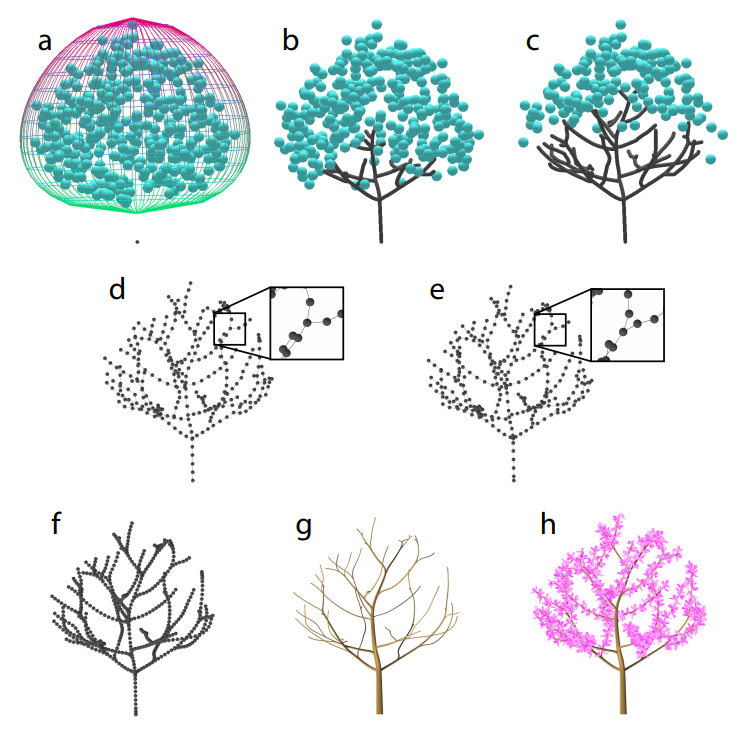
\includegraphics[scale=0.47]{AttractionPoints}
        \centering
\end{figure}

This is a very basic overview of course and I will research further into this method 
once I am sure of the scope and aim of the project. Whether I use this method or not 
however, I believe that this paper and it's references will be of great use moving 
forward.

\subsubsection{The Algorithmic Beauty of Plants}
This book \cite{beautyOfPlants} provides many insights into the algorithmic construction 
of plants. After a brief look through it seems that the most relevant section will be 
chapter 2 "Modeling of trees" which puts forward a method of generating branches through 
a \textit{mother branch} having two \textit{daughter branches} that split off from it. 
These daughter branches are shortened using constant ratios with repect to the mother 
branch and are angled from the mother branch using constant \textit{branching angles}. 
The mother branch and daughter branches are contained in the same \textit{branch plane}.

\begin{figure}[h]
        \caption{Proposed tree geometry}
        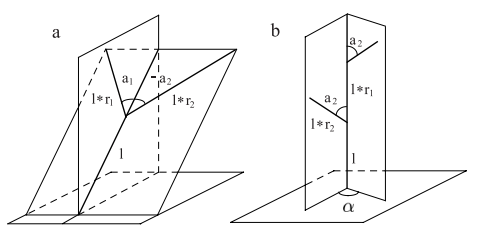
\includegraphics{MDbranches}
        \centering
\end{figure}

This book was co-authored by Przemysław Prusinkiewicz who was also a co-author of the 
space colonization paper I referenced previously. It seems that his research into 
the 3D construction of plants will be useful while researching for this project. 
Once I am sure of the direction I'm taking the project I will read into this book more 
closely to glean more details that could aid my progress.

\pagebreak
\section{Proposed Approaches}
My chosen approach for implementation will be using C++ to create an OpenGL module 
that can then be used as part of an existing OpenGL project. \\
At this early stage of the project I am unsure of the exact algorithmic method I 
will be using but I know the general process I will likely follow. \\
The tree trunk and branches will need to use some sort of random walk algorithm that 
takes into account the length and angle of growth of the parent branches. Some unit 
of randomness will have to be used to help produce realistic looking trees while 
following this process. Considering that I hope to create trees that will be seen to have grown 
around obstacles the random walk will also have to take obstacles into account and 
have a method to avoid them. \\
After the trunk and branches are fully constructed I will need a method of applying 
a correct thickness of the branches to the skeleton that I constructed using the 
random walk. I am currently unaware of whether it will be more beneficial to add 
thickness to the branches as the tree is constructed or if it will be easier to add 
after the entire skeleton is finished. \\
After the branches are finished completely I will need a method of adding leaves to 
the tree. Due to leaves only growing on further out branches I will need to have 
some method of distinguishing between the trunk of the tree and the branches. I don't 
know yet how I will add the leaves specifically. The likely approach would be to add 
a premade leaf model to parts of the branch using a chosen algorithm to decide their 
distribution. I have yet to fully understand the algorithms suggested in the paper I 
mentioned earlier \cite{colonization} but I will continue to research the possible 
methods.

\section{Risks, Mitigation and Contingency Planning}
Possible risks that could arise during this project are:

\begin{itemize}
        \item Loss of workstation (Laptop or PC). This will me mitigated through the 
              use of version control for both the codebase and report.
        \item Deletion of codebase from Github. This will be mitigated by having a 
              secondary physical backup of the codebase, allowing for it to be used 
              as a contingency plan in the event of the code being deleted.
        \item Scope creep is mitigated in the planning stage. I will follow a solid 
              plan that will allow me to reach realistic goals without the project 
              getting away from me.
\end{itemize}

\pagebreak
\begin{cmpfigure}{Project Gantt chart}
        \begin{sideways}
        \newganttchartelement{voidbar}{
        voidbar/.style={
        draw=black,
        top color=black!25,
        bottom color=black!23
        }}
        \begin{ganttchart}[x unit=0.45cm, vgrid, title label font=\scriptsize,
        canvas/.style={draw=black, dotted},
        /pgfgantt/milestone left shift = 0,
        /pgfgantt/milestone right shift = 0
        ]{1}{34}
        \gantttitle{Project schedule shown for e-vision week numbers
         and semester week numbers}{34} \\
        \gantttitlelist{9,...,42}{1}\\
        \gantttitlelist{1,...,12}{1}
        \gantttitle{CB}{4}
        \gantttitle{AS}{2}
        \gantttitlelist{1,...,8}{1}
        \gantttitle{EB}{4}
        \gantttitlelist{9,...,12}{1}\\
        
        
        %the elements, bars and milestones, are identified as elem0, elem1, etc
        
        %elem1
        \ganttbar{Project proposal}{1}{2}     \\  %elem0  
        \ganttbar{Literature review}{3}{6}    \\  %elem1 
        \ganttbar{Design}{6}{11}              \\  %elem2
        
        %week 1 of semester 2 is the 17th week in schedule 
        \ganttbar{Coding}{12}{12}                 %elem3
        \ganttvoidbar{}{13}{16}                   %elem4
        \ganttbar{}{17}{20}                   \\  %elem5
        
        \ganttbar{Testing}{12}{12}                %elem6
        \ganttvoidbar{}{13}{16}                   %elem7
        \ganttbar{}{17}{26}                    \\ %elem8
        \ganttmilestone{Code delivery}{26}    \\ %elem9
        \ganttbar{Final report writing}{25}{30}        \\ %elem10
        \ganttmilestone{Portfolio submission}{33}  \\ %elem11
        \ganttbar{Inspection preparation}{31}{34}  %elem12
        
        
        \ganttlink{elem0}{elem2} \ganttlink{elem1}{elem2} \ganttlink{elem2}{elem3}
        \ganttlink[link mid=.25]{elem2}{elem6} \ganttlink{elem5}{elem6}
        \ganttlink{elem8}{elem9} \ganttlink{elem9}{elem10}
        \ganttlink{elem10}{elem11} \ganttlink{elem11}{elem12}
        \end{ganttchart}
        \end{sideways}
\end{cmpfigure}

\clearpage
\bibliography{bibfile}
\end{document}